\chapter{Weighted Korn and Poincaré inequalities}   
\label{chap:wKorn}
\section{Introduction}
\begin{comment}
%\begin{com}TODO: Finish this

    Korn's inequalities in weighted spaces and Z2
-norms
were obtained earlier in the monograph [9] for bounded domains, and were
used by its author to study the smoothness of the solutions of the system of
elasticity theory.

This weight uses the distance of a point x to the clamped
part of the plate. Such a weight factor becomes a crucial tool in the derivation of an asymptotically sharp (with respect to the small parameter) form of Korn’s inequality for junctions
of thin plates (see [11]). Concerning junctions of massive bodies and thin rods we refer to
[2–5, 8–10, 12, 19, 24] and the review [23]. We emphasize that the final form of an asymptotically sharp weighted anisotropic Korn inequality is always very sensitive to the global
geometry of a junction including the type of boundary conditions.

Another aspect is that the classical Kotn’s first inequality requires
a least one condition on the displacement, such as a boundary or a normalization condition,
whereas the analogous geometric rigidity estimate does not. Therefore, in order to avoid the
imposed boundary conditions, one may be able to apply a localization argument in some
parts of the domain, by considering the analogous weighted version of the inequality under
consideration. Of course the last is a delicate question and is task for out future studies.

In the study of the asymptotic behavior of solutions to problems of elasticity theory in different thin
domains, it is necessary to consider weighted Korn’s inequalities since in thin plates and rods we must
distinguish between longitudinal and transverse directions.
\end{comment}

In this chapter, our focus shifts toward the exploration of Weighted Korn and Poincaré Inequalities, focusing on the theoretical underpinnings that lay the foundation for potential future applications. This segment is dedicated to broadening the scope of classical Korn inequality through its generalizations, a step crucial for laying the groundwork for future applied research. 

Several versions of weighted Korn and Poincaré inequalities, as explored in \cite{wKorn1,wKorn2,wKorn3,surveyQuasilinearSystems}, have proven to be extremely useful in various contexts. Firstly, they are indispensable when standard Cartesian coordinates are inadequate, and a shift to polar coordinates or other variable transformations is required. Additionally, the use of weights, particularly those based on the distance to boundary points, is essential for studying physical problems with clamped conditions, specifically in deriving asymptotically sharp forms of Korn’s inequality for junctions of thin plates and the study of junctions between massive bodies and thin rods. Lastly, classical Korn’s inequalities traditionally require at least one displacement condition, such as a boundary or normalization condition, unlike analogous geometric rigidity estimates. This difference opens the possibility of employing localization techniques in parts of the domain to bypass these conditions, particularly by leveraging the weighted version of the inequality—a strategy that presents a complex yet intriguing avenue for future research.


The journey begins with an examination of the generalizations of the classical Korn inequality. We shall introduce equations of the form:

$$
\|\delta_\GG(\Bx)^\alpha(\nabla \Bu-S)\|_{L^p(\Omega)} \leq  c(n,p,\alpha,L,R)\left\|\delta_\GG(\Bx)^\alpha e(\Bu)\right\|_{L^p(\Omega)}.
$$
and
$$
\|\delta'(\Bx)^\alpha(\nabla \Bu-R)\|_{L^p(\Omega)} \leq \frac{c(n,p,\alpha,L,R)}{h}\|\delta'(\Bx)^\alpha\operatorname{dist}(\nabla \Bu, \operatorname{SO}(n))\|_{L^p(\Omega)}.
$$
where  $\delta_\GG(\Bx)=\dist(\Bx, \partial\GG)$. The essence of this chapter lies in its subtle invitation to the reader to appreciate the intricate balance between abstract theoretical development and the anticipation of its eventual utility in solving real-world problems.

Most of the results were inspired by the paper of Sergi Conti and Barbara Zwicknagl, \cite{conti0}. In this paper it was proven a simpler weighed Poincaré inequality, which was crucial to a new proof of the Korn Inequality. In this chapter, we will use similar techniques to prove a stronger version of the weighted Poincaré inequality (\ref{sec:wPoincare}) that will imply a weighted version of the Korn inequality (\ref{sec:bulkWKorn}). Additionally, we will also introduce a new weighted Korn Inequality for plates in \ref{sec:plateWKorn}.

\section{Main results and Important Definitions}
\label{sec:mainWKorn}

 
    To be able to prove weighted Poincaré and Korn inequalities we need some conditions on the domain. In particular, we will need the domain to be uniformly Lipschitz.  We will use the definition used \cite{conti0} of uniformly Lipschitz domains:

\begin{definition}[Uniformly Lipschitz domains] \label{UniformLip} Let $L, R>0$. An open set $\Omega \subseteq \mathbb{R}^n$ is $(L, R)$-Lipschitz if there is $\Gve>0$ such that:
\begin{enumerate}
    \item $|\Bx-\By|<R\varepsilon$ for all $\Bx, \By \in \Omega$;
    \item For each $\Bx \in \partial \Omega$ there are $f_\Bx \in \operatorname{Lip}\left(\mathbb{R}^{n-1} ; \mathbb{R}\right)$ with $\operatorname{Lip}\left(f_\Bx\right) \leq L$ and an isometry $A_\Bx: \mathbb{R}^n \rightarrow \mathbb{R}^n$ such that $B_\varepsilon(\Bx) \cap \Omega=B_\varepsilon(\Bx) \cap V_\Bx$, where
        $$
            V_\Bx:=A_\Bx\left\{\left(\By^{\prime}, y_n\right) \in \mathbb{R}^{n-1} \times \mathbb{R}: y_n<f_\Bx\left(\By^{\prime}\right)\right\}
        $$
\end{enumerate}
\end{definition}
%\begin{lemma}[Whitney cover lemma] \label{Whitney} Given, $F\subset \R^n$, there exists  $x_1,x_2,\cdots \in F^c$, $r_1,r_2,\cdots\in \R$ defining a collection of balls $B_k=B(x_k,r_k)$ such that:
%\begin{enumerate}
%    \item The $B_k$ are pairwise disjoint.
 %   \item Let $B*_k= B(x_k,36r_k)$, then $\bigcup_k B*_k=F^c$.
 %   \item Let $B**_k= B(x_k,144r_k)$, then $B**_k\cap F \neq \emptyset$, for all $k$.
 %   \item $B*_k$ might not be disjoint, but they have the bounded intersection property.
%\end{enumerate}
%From properties 2 and 3 we can also conclude that for every k
%$$ 36 r_k\leq \dist(B_k,F)\leq 144r_k $$
%\end{lemma}
%\begin{question}
 %   Can we control the intersection in this case though? Doesn't look like it...
%\end{question}



So for uniform Lipschtiz domains, we can prove the Weighted Poincaré inequality and its respectively non-linear version, uniform rigidity:
\begin{theorem} [Weighted  Korn Inequality and Uniform Rigidity]\label{KornGamma} Let $\Omega \subset \mathbb{R}^n$ be a connected, bounded $(L, R)$-Lipschitz set,  $\GG$ an nonempty  close subset of $\dOm$ and $\delta_\GG(\Bx)=\dist(\Bx, \partial\GG)$. Then for any $\Bu \in W_{\mathrm{loc}}^{1, p}\left(\Omega ; \mathbb{R}^k\right)$, with $p \in[1, \infty)$, and every $\alpha\geq0$ there is are  $S \in \mathbb{R}_{\mathrm{skw}}^{n \times n}$ and $R \in \operatorname{SO}(n)$  such that
$$
\|\delta_\GG(\Bx)^\alpha(\nabla \Bu-S)\|_{L^p(\Omega)} \leq  c(n,p,\alpha,L,R)\left\|\delta_\GG(\Bx)^\alpha e(\Bu)\right\|_{L^p(\Omega)}.
$$
and
$$
\|\delta_\GG(\Bx)^\alpha(\nabla \Bu-R)\|_{L^p(\Omega)} \leq c(n,p,\alpha, L,R)\|\delta_\GG(\Bx)^\alpha\operatorname{dist}(\nabla \Bu, \operatorname{SO}(n))\|_{L^p(\Omega)}.
$$
\end{theorem}


%\begin{question}
%Will $c$ depend on $\GG$ and $\Ga$? Yes, do I need to specify the relation though?
%\end{question}

Additionally, we can prove similar results for plates $\Omega_h=\Omega\times I_h$, where the middle surface $\Omega$ satisfies the same condition as in the previous theorem.

\begin{theorem}[Weighted Korn Inequality and Uniform Rigidity for Plates] \label{KornGammaPlate} Let $\Omega_h=\Omega\times I_h \subset \mathbb{R}^3$ be a shell such that $\Omega$ is  a connected, bounded $(L, R)$-Lipschitz set and $I_h=[-h,h]$ for small $h>0$. Additionally, let $\delta'(\Bx)=\delta_{\dOm\times I_h}=\dist(\Bx,\dOm\times I_h)$ and $p \in(1, \infty)$. Then for any $\Bu \in W^{1, p}\left(\Omega_h ; \mathbb{R}^n\right)$ and any $\alpha\geq 0 $ , there are $R \in \operatorname{SO}(3)$ and $S \in \mathbb{R}_{\mathrm{skw}}^{3 \times 3}$ such that
$$
\|\delta'(\Bx)^\alpha(\nabla \Bu-S)\|_{L^p(\Omega)} \leq  \frac{c(n,p,\alpha,L,R)}{h}\left\|\delta'(\Bx)^\alpha e(\Bu)\right\|_{L^p(\Omega)}.
$$
and
$$
\|\delta'(\Bx)^\alpha(\nabla \Bu-R)\|_{L^p(\Omega)} \leq \frac{c(n,p,\alpha,L,R)}{h}\|\delta'(\Bx)^\alpha\operatorname{dist}(\nabla \Bu, \operatorname{SO}(n))\|_{L^p(\Omega)}.
$$
\end{theorem}


In order to prove these results, a new Weighted Poincaré inequality was necessary. Variations of Poincaré inequalities are important tools in proving the existence and uniqueness of several minimization problems, so we believe that this result deserves to be stated on its own.

\begin{theorem}[Weighted Poincaré Inequality] \label{WeightedPoincareOld} Let $\Omega \subset \mathbb{R}^n$ be a connected, bounded $(L, R)$-Lipschitz set,  $\GG$ an nonempty closed subset of $\dOm$  and $\delta_\GG(\Bx)=\dist(\Bx, \partial\GG)$. Then for any $\Bu \in W_{\mathrm{loc}}^{1, p}\left(\Omega ; \mathbb{R}^k\right)$, with $p \in[1, \infty)$, and every $\alpha\geq 0$ there is $\Ba \in \mathbb{R}^k$ such that:
    $$
    \|\delta_\GG(\Bx)^\alpha (\Bu-\Ba)\|_{L^p(\Omega)} \leq c(n,p,\alpha,L,R)\|\Gd_\GG(\Bx)^{1+\Ga} \nabla \Bu\|_{L^p(\Omega)} .
    $$
\end{theorem}

    \begin{remark}
    Theorems \ref{KornGamma} and \ref{WeightedPoincareOld} will be used several times for the particular case where $\GG=\dOm$. Additionally, for the last result, if we consider $\alpha=0$  we achieve the Weighted Poincare inequality \cite[Theorem~5.5]{conti0}, and since we have that $\delta_\GG\leq \operatorname{diam}(\Omega)$ the traditional inequality is also a corollary of this theorem. For both Korn inequalities, if we assume $\alpha=0$ we also get the traditional Korn inequality.
    \end{remark}
 
\section{Auxiliary Results and Lemmas}
\label{sec:auxWKorn}
The main results of this chapter are inspired by the proofs of \cite{conti0}, so the first step is to generalize Lemma 5.6 from that paper, which can be considered a Weighted Poincaré
  in 1D.

\begin{lemma}
\label{1dimPoinc}
Let $I=(a, b) \subseteq \mathbb{R}$ and  $E=[a,a+\epsilon]$ with $0<\epsilon< b-a$. For all $\varphi \in C^1(I),\alpha > 0 \in \mathbb{R}, A\in\R $ and   $p \in[1, \infty)$ we have that 
\begin{align*}
\int_I|(b-x)^\Ga(\phi-A)|^p d x &\leq 2^p \left(\frac{|I|}{|E|}\right)^{\alpha p+1}\int_E|(b-x)^\Ga(\beta-A)|^p d x\\ &\qquad+2^p \left(\frac{|I|}{|E|}\right)^{\alpha p+1}\left(\frac{p}{\alpha+1}\right)^p\int_I|(b-x)^{\Ga+1}\phi'|^p d x.
\end{align*}
\end{lemma}

\begin{proof} \textit{Step 1:}
Let $\beta = \phi(a)$, then by the fundamental theorem of calculus  applied to $(\phi-\beta)^p$ we get the following bound
$$|\phi-\beta|^p(x) \leq p \int_a^x|\phi(t)-\beta|^{p-1}\left|\phi^{\prime}(t)\right| d t .$$

Now if we multiply last equation by $(b-x)^{\alpha p}$ and integrate over $I$ we get

$$\int_I|(b-x)^\alpha(\phi-\beta)|^p(x) \leq p \int_I\int_a^x(b-x)^{\Ga p}|\phi(t)-\beta|^{p-1}\left|\phi^{\prime}(t)\right| d t dx.$$

Using Fubini's theorem we can conclude that
$$\int_I|(b-x)^\alpha(\phi-\beta)|^p(x) \leq \frac{p}{\Ga+1} \int_I(b-t)^{\Ga p+1}|\phi(t)-\beta|^{p-1}\left|\phi^{\prime}(t)\right| d t.$$

Since $\Ga p +1 = \Ga(p-1) + (1+\Ga)$, using Holder's inequality we  have that
$$\int_I|(b-x)^\Ga(\phi-\beta)|^p d x \leq \frac{p}{\alpha+1}\left\|((b-t)^\alpha(\phi(t)-\beta))^{p-1}\right\|_{L^{p^{\prime}(I)}}\left\|(t-b)^{1+\alpha} \phi^{\prime}(t)\right\|_{L^p(I)}.$$
where $p' = \frac{p}{p-1}$. Additionally, since  $$\left\|((b-t)^\alpha(\phi(t)-\beta))^{p-1}\right\|_{L^{p^{\prime}(I)}} = \left\|(b-t)^{\alpha}(\phi(t)-\beta)\right\|^{p-1}_{L^{p(I)}},$$ we can conclude the first step with the following inequality
\begin{equation}
\label{eq:step1}
\|(b-x)^\Ga(\phi-\beta)\|_{L^p(I)} \leq \frac{p}{\alpha+1}\left\|(b-x)^{1+\Ga} \phi^{\prime}\right\|_{L^p(I)}.
\end{equation}


\textit{Step 2:} Since we need to prove the inequality for any $A\in\R$ and not only $\beta$, the goal of this step is to analyze the integral of $|(b-x)^\Ga(\beta-A)|^p$.  Since $\beta$ and $A$ are constants we can compute  $\int_I|(b-x)^\Ga(\beta-A)|^p d x$ and $\int_E|(b-x)^\Ga(\beta-A)|^p d x$ exactly, and conclude that 
$$\frac{\int_I|(b-x)^\Ga(\beta-A)|^p d x}{\int_E|(b-x)^\Ga(\beta-A)|^p d x }=\frac{|I|^{\Ga+1}}{|E|^{\Ga+1}}\geq 1 ,$$ 
and consequently
$$\int_I|(b-x)^\Ga(\beta-A)|^p d x \leq \left(\frac{|I|}{|E|}\right)^{\Ga+1} \int_E|(b-x)^\Ga(\beta-A)|^p d x.$$



\textit{Step 3:} To conclude the proof we just need to apply triangular inequality two more times and use inequality \ref{eq:step1} 
\begin{align*}
    \int_I|(b-x&)^\Ga(\phi-A)|^p d x \leq 2^{p-1}\int_I|(b-x)^\Ga(\phi-\beta)|^p d x + 2^{p-1}\int_I|(b-x)^\Ga(\beta-A)|^p d x\\
     &\leq 2^{p-1}\int_I|(b-x)^\Ga(\phi-\beta)|^p d x + 2^{p-1}\left(\frac{|I|}{|E|}\right)^{\alpha p+1}\int_E|(b-x)^\Ga(\beta-A)|^p d x\\
     &\leq 2^p \left(\frac{|I|}{|E|}\right)^{\alpha p+1}\left(\int_E|(b-x)^\Ga(\phi-A)|^p d x+\int_I|(b-x)^\Ga(\phi-\beta)|^p dx \right)\\
    &\leq 2^p \left(\frac{|I|}{|E|}\right)^{\alpha p+1}\left(\int_E|(b-x)^\Ga(\phi-A)|^p d x+\left(\frac{p}{\alpha+1}\right)^p\int_I|(b-x)^{\Ga+1}\phi'|^p d x\right). 
\end{align*}
\end{proof}

The next step is to use the properties of uniformly Lipschitz domains and the previous result to prove something similar in higher dimensions, close to the boundary.

\begin{lemma}\label{PoincareBoundary}
     Let $\Omega \subset \mathbb{R}^n$ be $(L, R)$-Lipschitz, $\varepsilon$ as in Definition \ref{UniformLip}, $\Bx_* \in \GG\subset\dOm,\ r \in(0, \varepsilon /(4+$ $4 L)],\ p \in[1, \infty)$ and $\delta_\GG(\Bx)=\operatorname{dist}(\Bx, \GG)$. For any $u \in W_{\mathrm{loc}}^{1, p}(\Omega)$ there is $a \in \mathbb{R}$ such that
$$
\|\delta_\GG(\Bx)^\Ga (u-a)\|_{L^p(\Omega\cap B_r(\Bx_*))} \leq c(n,p,\Ga,L) \|\delta_\GG(\Bx)^{(\alpha+1)}\nabla u\|_{L^p(\Omega)}.
$$
\end{lemma}

\begin{proof}
    By the definition of $(L,R)-Lipschitz$ we have that $B\left(\Bx_*,\varepsilon\right) \cap \Omega=B\left(\Bx_*,\varepsilon\right) \cap V$, where 
$$
V:=A\left\{\left(\By^{\prime}, y_n\right) \in \mathbb{R}^{n-1} \times \mathbb{R}: y_n<f\left(\By^{\prime}\right)\right\},
$$ 
for an isometry  A  and an $L$-Lipschitz  function, $f$. Since all the results are invariant under rotation and translations we can, \textit{w.l.o.g.} assume that $A=I$, $\Bx_*=0$ and $f(\mathbf{0})=0$ to simplify the notation.

Let $\tau:= r L \in(0, \varepsilon / 4)$,  and consider the cylinder $T:=B_r^{\prime} \times(-3 \tau,-2 \tau)$ where $B'_r$ is the projection of $B_r(\Bx_*)$ into $x_n = 0$. For any $\Bx^{\prime} \in B_r^{\prime}$ we have $f\left(\Bx^{\prime}\right) \geq-r L=-\tau$, and therefore $4\tau\geq f\left(\Bx^{\prime}\right)-x_n \geq \tau$ for all $\left(\Bx^{\prime}, x_n\right) \in T$. Further, since $(3 h)^2+r^2 \leq (9L^2+1)r^2\leq \varepsilon^2$, we obtain that $T$  is still inside  $B_{\varepsilon} \cap V$ as we can see in the figure \ref{fig:wK}. 
\begin{figure}[!h]
    \centering
    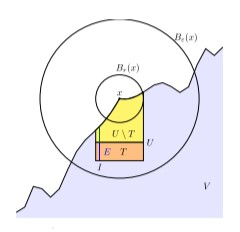
\includegraphics[scale = 2]{figures/wKornImage.jpg}
    \caption{Sketch of the geometry in the construction of Lemma \ref{PoincareBoundary}}
    \label{fig:wK}
\end{figure}

Additionally, since  $\operatorname{diam}(T)\leq c h$  by the usual Poincaré inequality there exist $a \in \mathbb{R}$ with
% so the shape of $T$ depends only on $A$ and $L$
\begin{align*}
\int_T|f(\Bx')-x_n|^{\alpha p}|u-a|^p d \Bx &\leq 4^{\Ga p} \tau^{\Ga p}\int_T|u-a|^p d\Bx\\
&\leq 4^{\alpha p} c(n,p,L) \tau^{(1+\alpha)p} \int_T|\nabla u|^p d \Bx\\
&\leq 4^{\alpha p} c(n,p,L) \int_T|f(\Bx')-x_n|^{(1+\alpha) p}|\nabla u|^p d \Bx.
\end{align*}

 For the next step we will apply Lemma \ref{1dimPoinc} to $u\left(\Bx^{\prime}, \cdot\right)$ for each $\Bx^{\prime} \in B_r^{\prime}$, with $I=\left(-3 \tau, f\left(\Bx^{\prime}\right)\right)$ and $E=(-3 \tau,-2 \tau)$. Since , $\tau=\mathcal{L}^1(E) \leq \mathcal{L}^1(I) \leq 4 \tau$, we get 
 \begin{align*}
\int_I|f(\Bx')-x_n|^{\alpha p}|u(\Bx',x_n)-a|^p d x_n &\leq c(n,p,\alpha,L)\int_I\left|f\left(\Bx^{\prime}\right)-x_n\right|^{(\alpha+1)p}|\nabla u|^p d x_n\\
&+c(n,p,\alpha,L) \int_E|f(\Bx')-x_n|^{\alpha p}|u(\Bx',x_n)-\alpha|^p d x_n.
\end{align*}

Let $U:=\left(B_r^{\prime} \times(-3 h, \infty)\right) \cap V$, so that $B_r(\Bx) \cap \Omega=B_r(\Bx_*) \cap U$ and $U \subseteq B_{\varepsilon}(\Bx_*) \cap V=B_{\varepsilon}(\Bx_*) \cap \Omega$ as we can see in the figure \ref{fig:wK}. We integrate over $\Bx^{\prime} \in B_r^{\prime}$, and use both of the above inequalities to conclude
$$
\begin{aligned}
\int_U|f(\Bx')-x_n|^{\alpha p}|u-\alpha|^p d \Bx & \leq c \int_{B_r^{\prime}} \int_I\left|f\left(\Bx^{\prime}\right)-x_n\right|^{(\alpha+1)p}|\nabla u|^p d x_n d \Bx^{\prime}\\
&\qquad \qquad + c \int_T\left|f\left(\Bx^{\prime}\right)-x_n\right|^{(\alpha+1)p}|\nabla u|^p d \Bx \\
& \leq c(\Ga,p,n,L) \int_U\left|f\left(\Bx^{\prime}\right)-x_n\right|^{(\alpha+1)p}|\nabla u|^p d \Bx.
\end{aligned}
$$
Additionally, by construction of $U$ we have that $|f\left(\Bx^{\prime}\right)-x_n|$ is comparable with $\delta(\Bx)$. In ~\cite[Lemma5.7]{conti0} it is proven that there exists $c(L)>0$, such that
$$
\left|f\left(\Bx^{\prime}\right)-x_n\right| \leq c(L) \delta_\dOm(\Bx)\leq c(L)\delta_\GG(\Bx) \quad \text { for all }\quad \Bx \in U ,
$$
and for a lower bound, we use the fact that $\Bx^*\in \GG$ to get
\begin{align*}
    \Gd_\Gamma(\Bx)\leq \dist(\Bx,\Bx^*)
    \leq\sqrt{9\tau^2+r^2}
    =\sqrt{9L+1}r
    \leq \frac{\sqrt{9L+1}}{L} |f\left(\Bx^{\prime}\right)-x_n|,
\end{align*}
so in fact there exist $c(L)$ such that
$$\frac{1}{c(L)} \delta_\GG(\Bx)\leq \left|f\left(\Bx^{\prime}\right)-x_n\right| \leq c(L) \delta_\GG(\Bx) \quad \text { for all }\quad \Bx \in U .$$
which concludes the proof since $B_r(\Bx_*) \cap V \subseteq U$.
\end{proof}

Finally, to put all these pieces together we will need Whitney Covering Lemma. A more general version of the lemma can be seen in \cite{stein}, but for simplicity, we will introduce the necessary statement for our framework:

\begin{lemma}[Whitney covering lemma] \label{Whitney}Let $\GG\in \mathbb{R}^n$ be a closed non-emptyset set. We can cover $\GG^c$ by a collection of closed cubes $Q_j$ that are essentially disjoint, and whose size is comparable to their distance from $\GG$, $i.e$
    \begin{enumerate}
    \item $\cup_j Q_j=\GG^c$ and  $Q_j$ 's have disjoint interiors,
    \item $\sqrt{n} \ell\left(Q_j\right) \leq \operatorname{dist}\left(Q_j, \GG\right) \leq 4 \sqrt{n} \ell\left(Q_j\right)$,
    \item If the boundaries of two cubes $Q_j$ and $Q_k$ touch then $\frac{1}{4} \leq \frac{\ell\left(Q_j\right)}{\ell\left(Q_k\right)} \leq 4$,
    \item For a given $Q_j$ there exist at most $12^n Q_k$ 's that touch it.
    \end{enumerate}
    Where $\ell(Q)$ denotes the length of a cube $Q$.
    
    Additionally, we can also conclude that $2Q_j\subset \GG^c$ and that the cover $\{2Q_j\}_j$ has the finite overlap property.
    \end{lemma}
    \begin{remark}
        This Lemma is often used to cover an open set $\Omega\in \R^n$ by choosing $\GG=\dOm$ and restricting only to the cubes inside $\Omega$.
    \end{remark}

    We will notice that part of our cover will be outside of $\Omega$. Since our functions are just defined in $\Omega$ to handle this problem we will consider the following extension from ~\cite[Theorem~4.7]{evansGa}. 
    \begin{lemma}\label{GradExt} Let $\Omega$ be a $(L, R)$-Lipschitz domain and $\Bu\in W^{1,p}(\Omega,\mathbb{R}^k)$, with $p\in[1,\infty)$, then there exists a gradient preserving extension $\tilde{\Bu}\in W^{1,p}(\R^n,\R^k)$, i.e.,
    $$\|\nabla(\tilde{\Bu})\|_{L^p(\R^n)}\leq c(n,L,R)\|\nabla(\Bu)\|_{L^p(\Omega)},$$ 
    and
    $$\tilde{\Bu}(\Bx)=u(\Bx) \quad \text { for all } \Bx \in \Omega.$$
    \end{lemma}

    \begin{comment}
        is this necessary?
    \end{com}
    \begin{lemma} \label{EnergyExt}Let $\Omega$ be a $(L, R)$-Lipschitz domain and $u\in W^{1,p}(\Omega)$ then there exists a energy preserving extension $\tilde{u}\in W^{1,2}(\R^n)$, i.e.,
    $$\|E(\tilde{u})\|_{L^2(\R^n)}\leq c(n,L,R)\|E(u)\|_{L^2(\Omega)}$$
    and
    $$\tilde{u}(x)=u(x) \quad \text { for all } x \in \Omega$$
    \end{lemma}
\end{comment}
    

\section{ Proof of Weighted Poincare inequality for bulk domains}
\label{sec:wPoincare}
In this section, we will prove the weighted Poincaré inequality \ref{WeightedPoincareOld}. The proof is harder than the one in \cite{conti0} since a Vitali's cover is not sufficient, in our case, we will need to apply a Whitney cover for the interior and a Vitali's cover close to $\GG$.
%\begin{theorem}[Weighted Poincaré] \label{WeightedPoincare} Let $\Omega \subseteq \mathbb{R}^n$ be a connected, bounded $(L, R)$-Lipschitz set,  $\GG$ an nonempty closed subset of $\dOm$  and $\delta_\GG(x)=\dist(x, \partial\GG)$. Then for any $u \in W_{\mathrm{loc}}^{1, p}\left(\Omega ; \mathbb{R}^k\right)$, with $p \in[1, \infty)$, and every $\alpha\geq0$ there is an  $a \in \mathbb{R}^k$ such that:
%$$
%\|\delta_\GG(x)^\alpha (u-a)\|_{L^p(\Omega)} \leq c(n,p,\alpha,L,R)\|\Gd_\GG(x)^{1+\Ga} \nabla u\|_{L^p(\Omega)} .
%$$
%In particular, $u \in L^p\left(\Omega ; \mathbb{R}^k\right)$. 
%\end{theorem}
\begin{proof}[Proof of Theorem \ref{WeightedPoincareOld}]
First notice that it suffices to consider the scalar case, additionally, using a density argument we can also assume $u$ in $C^1(\Omega)$. For brevity, let $A:=\|\delta_\GG(\Bx)^{1+\alpha} \nabla u\|_{L^p(\Omega)}$. Let $\varepsilon$ be as in Definition \ref{UniformLip} and fix $r_B:=\varepsilon /(12(L+1))$ (the reason will become clear below). 

\textit{Step 1:} Let's start by using a Vitali's cover $\Gamma_{2r_B} := \{\Bx\in \Omega\ :\ \delta_\GG(\Bx)\leq 2r_B\} $ with  balls of radius $4Lr_B$ and centers $\Bx^i$, \textit{i.e.}:
$$\mathcal{U}^\GG= \{ B^\GG_i := B_{4Lr_B}(\Bx^i)\cap \Omega,\ \Bx^0,\ldots, \Bx^K \in \GG,\ |\Bx^i-\Bx^{i-1}|< \frac{r_B}{L}\}.$$

\textit{Claim: There exist $c(n,L)$ such that, for each $i=1,\cdots, K$, we have that
$$|B^\GG_i\cap B_{i-1}^\GG\cap \GG^c_{r_B}|\geq c(n,L) r_B^n\quad \text{and}\quad \|\delta_\GG(\Bx)^\alpha\|^p_{L^p \left(B^\GG_{i}\cap B^\GG_{i-1}\right)}\geq c_L r_B^{n+\alpha p}. $$}

First of all, we can, \textit{w.l.o.g.}, consider $L\geq 1$ so we have that $B^\GG_i\cap B_{i-1}^\GG\subset B_\varepsilon(\Bx^i)$. Additionally, to simplify the proof, we can consider $\Bx^i=(\Bx^{i'},x^i_n),$ $f_{\Bx^i}(\Bx^{i'})=0,\ f_{\Bx^{i}}(\Bx^{i-1'})\geq 0$ and $A_{\Bx^i}=I$.

Let $m_i = \min_{B_{r_B/L}(\Bx^{i'})} f_{\Bx^i}(\Bx')$, since $f_{\Bx^i}$ is a $L-$lipschitz function we have that
$$m_i \geq - r_B\quad\text{and}\quad f_{\Bx^{i}}(\Bx^{i-1'})\leq r_B.$$
 So, in fact the intersection is minimized when  $\Bx^{i-1}=(\By',y_n)= (\Bx^{i'}+\frac{r_B}{L}\frac{\Bx^{i-1'}-\Bx^{i'}}{|\Bx^{i-1}-\Bx^{i'}|},r_B)$, which implies that
\begin{align*}
    B^\GG_i\cap B^\GG_{i-1}\cap\GG^c_{r_B}&\supset
     B^\GG_i\cap B^\GG_{i-1}\cap \{(\Bx',x_n): \Bx'\in B_{r_B/L}(\Bx^i)\ \wedge\  x_n\leq m_i-r_B\}\\&\supset
    B^\GG_i\cap B_{4Lr_B}(\By)\cap \{(\Bx',x_n): \Bx'\in B_{r_B/L}(\Bx^i)\ \wedge\  x_n\leq m_i-r_B\}.
\end{align*}
Additionally, the cylinder $$C_\By = B(\Bx^{i'},\frac{r_B}{L})\times \left[\left(-4\sqrt{1-\frac{r_B}{4L^2}}+1\right)r_B,m_i-r_B\right],$$ is  also included in the intersection, so
\begin{align*}
    |B^\GG_i\cap B_{i-1}^\GG\cap \GG^c_{r_B}|&\geq |C_\By|\\
    &\geq \omega(n-1)\left(\frac{2r_B}{L}\right)^{n-1}\left[\left(4\sqrt{1-\frac{r_B}{4L^2}}-1\right)r_B+m_i-r_B\right]\\
        & \geq \omega(n-1)\left(\frac{2}{L}\right)^{n-1}\left(4\sqrt{1-\frac{1}{4L^2}}-3\right)r_B^n. 
\end{align*}
So the claim is proven, with $c(n,L) =\omega(n-1)\left(\frac{2}{L}\right)^{n-1}\left(4\sqrt{1-\frac{1}{4L^2}}-3\right)$, where $\omega(n)$ is the volume of the unit ball in $\mathbb{R}^n$.


Additionally, we can conclude that
\begin{align*}
   \|\delta_\GG(\Bx)^\alpha\|^p_{L^p \left(B^\GG_{i}\cap B^\GG_{i-1}\right)}&\geq r_B^{\alpha p} |B^\GG_i\cap B^\GG_{i-1}\cap \GG^c_{r_B}|\\
   &\geq c_L r_B^{n+\alpha p}. 
\end{align*}


\textit{Step 2:} To work away from $\GG$ we will consider the Whitney cover, $\{\hat{Q}_j\}_{j\in \mathbb{N}}$ of the open set $\GG^c$ defined in the Lemma \ref{Whitney}. More precisely, we consider the  cubes centered in $\Bx^j$, $\hat{Q}_j := \Bx^j + (-r_j,r_j)^n$ from the Whitney cover and the bigger cubes $Q_j := \Bx^j + (-\frac{3}{2}r_j,\frac{3}{2}r_j)^n $. Additionally we will consider only the sub-cover of  $\{Q_j\}_{j\in \mathbb{N}}$ such that the respective $\hat{Q}_j$ intersects $\Omega\cap\GG^c_{r_B}$, i.e,

$$\mathcal{U}^{int}:= \{Q_j^{int}:=Q_j,\ \hat{Q}_j\cap\Omega\cap\GG_{r_B}^c\neq \emptyset \}.$$
  
For a better understanding of this cover, we can go over its  main properties:
\begin{enumerate}
    %\item $\Omega\cap\GG^c_{r_B}\subset\bigcup_j Q^{int}_{j}$ and the $\hat{Q}^{int}_{j}$ 's have disjoint interiors.
    \item $2\sqrt{n} r_j \leq \delta_\GG(\hat{Q}^{int}_{j}) \leq 8 \sqrt{n} r_j$ and $\frac{3\sqrt{n}}{2} r_j \leq \delta_\GG(Q^{int}_{j}) \leq 6 \sqrt{n} r_j$, 
\item If the boundaries of two cubes $\hat{Q}^{int}_{j}$ and $\hat{Q}^{int}_{i}$ touch then $\frac{1}{4} \leq \frac{r_j}{r_i} \leq 4$,
\item For a given $Q^{int}_{j}$, it intersect a finite number of $Q^{int}_i$ 's,
\item For every $j$, we have that $r_j\geq\frac{r_B}{\sqrt{n}}$,
\item The cover is finite, so, after rearranging we can consider  $j=0,1,\cdots =J$ for some $J\in \mathbb{N}$.
\end{enumerate}

%However we are looking for an overlapping cover, so let $x^{K+j'}$ be the center of the square $Q_{j'}$, $r_{K+j'}= 2\ell(Q_{j'})$, and let's add to our previous collection the balls $B_{K+j'}=B(x^{K+j'},r_{K+j'})$, which satisfy $$\frac{(\sqrt{n}-1)}{2} r_{K+j'} \leq \delta_\GG(B_{K+j'}) \leq 2 \sqrt{n} r_{K+j'}$$

Similar to the previous claim we would like to be able to control the size of the intersection of 2 cubes in this cover. In fact, we will just need to do it when $\hat{Q}^{int}_{j}$ and $\hat{Q}^{int}_{i}$ are adjacent. \textit{W.l.o.g.} we can assume that $\ell(\hat{Q}^{int}_{j})\leq \ell(\hat{Q}^{int}_{i}) $. Then
$$|{Q}^{int}_{j}\cap {Q}^{int}_{i}|\geq \frac{1}{2}|\hat{Q}^{int}_{j}| =\frac{1}{2} (2 r_j)^n.$$

Lastly, is important to remark that this cover actually covers more than $\Omega$, but $u$ is just defined in $\Omega$. To overcome this problem we can use the gradient preserving extension, $\tilde{u}$, defined in Lemma \ref{GradExt}. To keep the notation simple we will still use $u$ instead of $\tilde{u}$, but we will keep in mind that we can consider $u$ to be defined in $\R^n$ when necessary.


\textit{Step 3:} The next step is to understand how both covers interact, so it will be useful to merge and relabel them. Let $$\Omega^{ext}=\bigcup_{j=0}^K B^\GG_j\bigcup_{j=0}^J Q^{int}_j,$$ and it's cover $$\mathcal{U}=\{B_j:=B^\GG_j,\ j =0,\ldots, K\ B_{K+j}:=Q^{int}_j,\ j=0,\ldots, J\}.$$ 

%TODO>    Would it make it easier to read if both covers were balls or cubes?

To move from the inside to the outside cover we need to be able to control the size of the intersection for some interior ball $B_{K+j}$ and boundary ball $B_k$. This will not be possible for every intersecting ball, so let's assume that the respective smaller cuber, $\hat{Q}^{int}_{j}$ intersects $\GG_{r_B}$. Thisthat $\Bx_{K+j}\in \GG_{2r_B}$, so there must be a boundary ball containing $\Bx_{K+j}$, let's make it $B_k$.

By property 4 of the Whitney cover,  $r_{K+j}\geq \frac{r_B}{\sqrt{n}}$, we have the desired bounds:
$$|B_{K+j}\cap B_{k}|\geq c(L,n) r^n_B,\text{   and   }  \|\delta_\GG(\Bx)^\alpha\|^p_{L^p \left(B_{K+j}\cap B_{k}\right)}\geq c(n,L) r_{K+j}^{n+\alpha p }.$$

\textit{Step 4:} To understand why we built our cover this way we will see that in fact we can prove a weighted Poincare in each set $B_j,\ j =1,\ldots, K+J$.  For $j\leq K$ we can use Theorem \ref{PoincareBoundary} to conclude that there exist $a_j\in \R$ such that
$$
\|\delta_\GG(x)^\alpha (u-a_j)\|_{L^p\left(B_j\cap \Omega\right)} \leq c(n,p,\Ga,L) A,
$$

and for $j>K$  we can apply the standard poincaré inequality and property 1, to obtain $a_j$:
\begin{align*}
    \|\delta_\GG(\Bx)^\alpha (u-a_j)\|_{L^p\left(B_j\right)} &\leq (4\sqrt{n}r_j)^\alpha\| (u-a_j)\|_{L^p\left(B_j\right)}\\
    &\leq c(n,p,\alpha,L)r_j^\alpha\| \nabla u\|_{L^p\left(B_j\right)}\\
    &\leq c(n,p,\alpha,L) \|\delta_\GG(\Bx)^\alpha \nabla u\|_{L^p\left(B_j\right)}.
\end{align*}

\textit{Step 5:} The main problem is that for each different set, we have a different constant $a_j$, so we need to find a way to control the size of $a_j$ when we move from one set to another. Fix $k\in \{0,1\ldots K+J\}$, and consider the sequence $j_0:=0, j_1, \ldots, j_H:=k$ such that $B_{j_h} \cap B_{j_{h+1}} \cap \Omega \neq \emptyset$ for all $h$. This is possible since $\Omega^{ext}=\cup B_k\cap \Omega\bigcup\cup B_{K+j'}$ is connected, which means that there is a continuous curve in $\Omega^{ext}$ which joins a point $\Bx^0$ and $\Bx^k$; as the curve is compact it is covered by finitely many of the balls. We can further assume, by step 1,2,3,  that:
\begin{comment}:
\begin{enumerate}
    \item the indices $j_h$ to be distinct. Indeed, if $j_h=j_{h^{\prime}}$ for some $h<h^{\prime}$, we can remove $h, h+1, \ldots, h^{\prime}-1$ from the set.
    \item if $j_h,j_{h+1}\leq K$ then we can consider $j_{h+1}=j_h\pm 1$
    \item if $j_h,j_{h+1} > K$ then we can consider that the boundary of $\hat{Q}_{j_h-K}$ and $\hat{Q}_{j_{h+1}-K}$ touch.
    \item if $j_h\leq K< j_{h+1}$ then $\Bx_{j_{h+1}}\in B_{j_h}$
\end{enumerate} 
\end{comment}
$$  \|\delta_\GG^\alpha(\Bx)\|_{L^p \left(B_{j_{h+1}} \cap B_{j_{h}}\right)}\geq c(n,p,L) r_{j_h}^{n/p+\alpha }.$$
Using the last inequality we can then control the size of $|a_{j_{h}}-a_{j_{h+1}}|$:
\begin{align*}
    r_{j_h}^{n / p+\alpha}|a_{j_{h}}-a_{j_{h+1}}| &\leq
    c \|\delta_\GG^\alpha(\Bx)\|_{L^p \left(B_{j_{h+1}} \cap B_{j_{h}}\right)}|a_{j_{h}}-a_{j_{h+1}}|\\
    &\leq c\|\delta(\Bx)^\alpha(a_{j_{h}}-a_{j_{h+1}})\|_{L^p \left(B_{j_{h+1}} \cap B_{j_{h}}\right)}\\
    &\leq c \|\delta(\Bx)^\alpha(u-a_{j_{h}})\|_{L^p \left(  B_{j_{h}}\right)}+ \|\delta(\Bx)^\alpha(u-a_{j_{h+1}})\|_{L^p \left(B_{j_{h+1}}\right)}\\
    & \leq c(n,p,\alpha,L) A.
\end{align*}



\textit{Step 5:} To finalize, for each $B_k$ we can always  create a finite path that starts at $B_0$ and finishes at $B_k$. Besides that the size of all the balls are comparable, i.e., there exist $C=C(L,R)$ such that $\frac{1}{C}\leq\frac{r_{k_1}}{r_{k_2}}\leq C$ for every $k_1,k_2\in[0, K+J]$. So taking $a=a_0$ we have that
\begin{align*}
\left\|\delta(\Bx)^\alpha (u-a)\right\|_{L^p(\Omega)} &\leq \sum_{k=0}^{K+J}\left\|\delta(\Bx)^\alpha (u-a_0)\right\|_{L^p(B_k\cap \Omega)}\\
&\leq\sum_{k=0}^{K+J}\left[\left\|\delta(\Bx)^\alpha (u-a_k)\right\|_{L^p(B_k)}+\left\|\delta(\Bx)^\alpha (a_k-a)\right\|_{L^p(B_k)}\right]\\
&\leq C(K+J) A +\sum_{k=0}^{K+J}\sum_{h=0}^{H_k} \left\|\delta(\Bx)^\alpha (a_{j_{h+1}}-a_{j_h 
 }) \right\|_{L^p(B_k)}\\ 
 &\leq C(K+J) A+\sum_{k=0}^{K+J}\sum_{h=0}^{H_k}c r_k^{n/p+\alpha}\left|a_{j_{h+1}}-a_{j_h 
 }\right|\\
 & \leq C(n,p,\alpha,L,R)  A, 
\end{align*}
as desired. 
\end{proof}

\begin{remark} Even if $u=0$ in $\GG$ we can't assume that $a=0$ as usual in other poincaré inequalities. This happens because even to control the function near the boundary we always use information from the interior. To confirm this we can look at the following 1d counter-example, for $\Omega =[0,1]$ and $\GG=\{0\}$. Take
$$u_n=\begin{cases} n\ if\  \delta_\GG(x)\geq \frac{1}{n}\\
\delta_\GG(x)n^{2}\  if \  \delta(x)\leq \frac{1}{n} \end{cases}\qquad |u'_n| = \begin{cases} 0\ if\  \delta_\GG(x)> \frac{1}{n}\\
n^{2}\  if \  \delta_GG(x)\leq \frac{1}{n} \end{cases}
$$

So for $n>4$ we have that 

$$\int_0^1 \delta_\GG(x)^{\alpha p} u_n(x) ^p \geq \int_{\delta_\GG(x)\geq 1/4} \delta_\GG(x)^{\alpha p}n^p \geq \frac{1}{4^{\alpha p}}\frac{1}{2}n^p\to \infty$$

However $$\int_0^1 \delta_\GG(x)^{(\alpha+1) p} |u'_n(x)| ^p = \int_0^{\frac{1}{n}} x^{(\alpha+1)p} n^{2p} =\frac{2}{(\alpha+1)p+1}n^{2p-(\alpha+1)p-1} =C n^{p(1-\alpha )-1} $$


so we conclude that for any $p>0, \alpha>0$ 

$$\frac{\|\delta(x)^\alpha |u_n(x)|\|^p}{\|\delta(x)^{\alpha+1} |u'_n(x)|\|^p}\geq C \frac{n^p}{n^{p(1-\alpha)-1}}=n^{1+p\alpha}  \to \infty$$

So there is no guarantee that $a=0$  even if it vanishes on $\GG$.

\end{remark}
\section{Weighted Korn inequality for a bulk domain}
\label{sec:bulkWKorn}

In this section, we will prove the weighted Korn inequality \ref{KornGamma}. The idea is very similar to the proof of the weighted Poincaré inequality (Theorem \ref{WeightedPoincareOld}), but we can use a simpler cover. Results like this normally are proved for $\GG=\dOm$, but we will prove it for a more general $\GG$ because it will be necessary to prove the result for plates.
\begin{comment}
\begin{theorem}\label{KornGamma}
(Uniform rigidity) Let $\Omega \subseteq \mathbb{R}^n$ be a connected, bounded $(L, R)$-Lipschitz set, $p \in(1, \infty)$ and $\GG\subset \partial\Omega$ a non empty close set. Then for any $u \in W^{1, p}\left(\Omega ; \mathbb{R}^n\right)$ there are $R \in \operatorname{SO}(n)$ and $A \in \mathbb{R}_{\mathrm{skw}}^{n \times n}$ such that
$$
\|\delta_\GG(x)^\alpha(\nabla u-A)\|_{L^p(\Omega)} \leq c_{\operatorname{Rig}}\left\|\delta_\GG(x)^\alpha(\nabla u+\nabla u^T)\right\|_{L^p(\Omega)}
$$
and
$$
\|\delta_\GG(x)^\alpha(\nabla u-R)\|_{L^p(\Omega)} \leq c_{\mathrm{Rig}}\|\delta_\GG(x)^\alpha\operatorname{dist}(\nabla u, \operatorname{SO}(n))\|_{L^p(\Omega)}.
$$

The constant $c_{\text {Rig }}$ depends only on $n, p, L$ and $R$.
\end{theorem}
\end{comment}
\begin{proof}[Proof of Theorem \ref{KornGamma}]
  
    When $\Omega$ is a cube and $\alpha=0$ both of these results are well known (Theorem \ref{KornGeneralDomain}, \ref{uniformRigidityGeneral} ), and the technique to extend to the general equation is identically in both cases so we will just prove the second inequality.

    Contrary to the proof of the weighted Poincaré Inequality, for this theorem, we do not need a different cover near $\GG$, we will just use the  Whitney cover  from  lemma \ref{Whitney}:
    
    $$\mathcal{U}:= \{Q_j,\ \hat{Q}_j\cap\Omega\neq \emptyset,  \ j=0,\ldots,J \},\qquad \Omega^{ext}= \cup_j \hat{Q}_j.$$

    As in the previous theorem, we will use the gradient preserving extension, $\tilde{\Bu}$, defined in Lemma \ref{GradExt}, while still using $\Bu$.
    
    \textit{Step 1:} The first step is to apply the normal Uniform Rigidity inequality to each cube in the cover. So for each $Q_j$ we have that there exist $R_j\in SO(n)$ such that
    \begin{align*}    
        \left\|\delta_\GG(\Bx)^\alpha\nabla (\Bu-R_j)\right\|_{L^p(Q_j)} & \leq (4\sqrt{n} r_j)^\alpha \left\|\nabla (\Bu-R_j)\right\|_{L^p(Q_j)}\\ &\leq C (4\sqrt{n} r_j)^\alpha \left\|\operatorname{dist}\left(\nabla \Bu, \mathrm{SO}(n)\right)\right\|_{L^p(Q_j)}\\
        &\leq C(n,p,\alpha)  \left\|\delta_\GG(\Bx)^\alpha \operatorname{dist}\left(\nabla \Bu, \mathrm{SO}(n)\right)\right\|_{L^p(Q_j)}.
    \end{align*}

    Notice that since all the sets are cubes, the constant $C(n,p,\Ga)$ is the same for every $j$.
    
    \textit{Step 2:} Again, we have a different constant for each cube, but this time to find the right constant we will use a different technique.  Let start by constructing a partition of unity subordinated to $\CU$,  i.e., fix $\varphi^* \in C_c^{\infty}\left((-1,1)^n ;[0,1]\right)$ with $\varphi^*=1$ on $\left(-\frac{1}{2}, \frac{1}{2}\right)^n$, let $\hat{\varphi}_j(\Bx):=\varphi^*\left(\left(\Bx-\Bx^j\right) / 2r_j\right)$ and $\varphi_j:=\hat{\varphi}_j / \sum_k \hat{\varphi}_k$ which is well define in $\Omega^{ext}$ since there is at least one $\hat{\varphi}_k>0$, so it have the following properties:
    \begin{enumerate}
            \item $\varphi_j \in C_c^{\infty}\left(Q_j\cap \Omega^{ext}\right)$,
            \item $ \sum_j \varphi_j=1$ in $\Omega^{ext}$,
            \item $\left|\nabla \varphi_j\right| \leq c / r_j$. 
    \end{enumerate}

Then we can define  a smooth interpolation  of all $R_j$ defined in $\Omega^{ext}$, $$\beta:=\sum_j \varphi_j R_j.$$ 

Since the overlap of the sets is finite, by the properties of the partition of unity we have that:
\begin{align*}
\|\delta_\GG(\Bx)^\alpha(\nabla \Bu-\beta)\|_{L^p(\Omega)}&=\left\|\delta_\GG(\Bx)^\alpha\sum_j \varphi_j\left(\nabla u-R_j\right)\right\|_{L^p(\Omega)} \\ &\leq C \sum_j\left\|\delta_\GG(\Bx)^\alpha(\nabla \Bu-R_j)\right\|_{L^p\left(Q_j\right)} \\
& \leq  C(n,p) \left\|\delta_\GG(\Bx)^\alpha \operatorname{dist}(\nabla \Bu, \mathrm{SO}(n))\right\|_{L^p\left(\Omega\right)} .
\end{align*}

\textit{Step 3:} This looks similar to what we need to prove, however, $\beta$ is not constant, so we will have to apply weighted Poincaré inequality proved in  \ref{WeightedPoincareOld}. To do so, we will need to control the size of the gradient of $\beta$. Since, $\sum_j \nabla \varphi_j=0$ on $\Omega$ we have that
$$
\nabla \beta=\sum_j \nabla \varphi_j R_j=\sum_j \nabla \varphi_j\left(R_j-\nabla \Bu\right) \text {. }
$$
Additionally, recall that $\left|\nabla \varphi_j\right| \leq C / r_j$, and that $\delta_\GG\left(Q_j\right) \leq C r_j$, which implies that
$$
\delta_\GG(\Bx)\left|\nabla \varphi_j\right|(\Bx) \leq C \chi_{Q_j}(\Bx) \quad \text { for all } \Bx \in \Omega .
$$
Therefore
$$
\begin{aligned}
\|\delta_\GG(\Bx)^{(1+\alpha)}\nabla \beta\|_{L^p(\Omega)} & \leq C \sum_j \|\delta_\GG(\Bx)^{(1+\alpha)}\nabla \varphi_j\left(\nabla \Bu-R_j\right)\|_{L^p(Q_j)} \\
& \leq C(n,p,\alpha) \sum_j \|\delta_\GG(\Bx)^{\alpha}\left(\nabla \Bu-R_j\right)\|_{L^p(Q_j)}.
\end{aligned}
$$
So, by applying the weighted Poincaré inequality to $\beta$, we obtain  $R_* \in \mathbb{R}^{n \times n}$, such that
\begin{align*}
\left\|\delta_\GG(\Bx)^{\alpha}(\beta-R_*)\right\|_{L^p(\Omega)} &\leq C \|\delta_\GG(\Bx)^{(1+\alpha) }\nabla \beta\|_{L^p(\Omega)}\\
 &\leq C(n,p,\alpha,L,R)\|\delta_\GG(\Bx)^{\alpha}\operatorname{dist}(\nabla \Bu, \mathrm{SO}(n))\|_{L^p(\Omega)}.
\end{align*}

\textit{Step 4:} The last problem that needs to be fixed is that $R_*$ is not necessarily in $\operatorname{SO}(n)$.Although,  $\operatorname{SO}(n)$ is compact, so we can take  $R$ be the closest matrix to $R_*$ in $\operatorname{SO}(n)$, which satisfies:
$$\left|R-R_*\right|=\operatorname{dist}\left(R_*, \mathrm{SO}(n)\right) \leq\left|R_*-\nabla \Bu\right|(\Bx)+\operatorname{dist}(\nabla \Bu(x), \mathrm{SO}(n)),$$
for every $\Bx$. So we can conclude that
\begin{align*}
\|\delta_\GG(\Bx)^\alpha(\nabla \Bu-R)\|_{L^p(\Omega)}&\leq \|\delta_\GG(\Bx)^\alpha(\nabla \Bu-R_*)\|_{L^p(\Omega)}+\|\delta_\GG(\Bx)^\alpha(R_*-R)\|_{L^p(\Omega)}\\
&\leq 2\|\delta_\GG(\Bx)^\alpha(\nabla \Bu-R_*)\|_{L^p(\Omega)} +\|\delta_\GG(\Bx)^\alpha \operatorname{dist}(\nabla \Bu, \mathrm{SO}(n))\|_{L^p(\Omega)}\\
&\leq 2\|\delta_\GG(\Bx)^\alpha(\nabla \Bu-\beta)\|_{L^p(\Omega)} + 2\|\delta_\GG(\Bx)^\alpha(\beta-R_*)\|_{L^p(\Omega)}\\
&\qquad\qquad +\|\delta_\GG(\Bx)^\alpha \operatorname{dist}(\nabla \Bu, \mathrm{SO}(n))\|_{L^p(\Omega)}\\ 
&\leq C(n,p,\alpha,L,R) \|\delta_\GG(\Bx)^\alpha \operatorname{dist}(\nabla \Bu, \mathrm{SO}(n))\|_{L^p(\Omega)},
\end{align*}
as desired.

\end{proof}

\section{Weighted Korn Inequality for Plates}
\label{sec:plateWKorn}

Theoretically, the previous result is also true for plates, however, to be able to control the size of the constant when the thickness of the plate goes to zero we need a different approach.

\begin{proof}[Proof of Theorem \ref{KornGammaPlate}]
Again we will just need to focus on one of the inequalities, this time we will just prove the first one. Similar to the proof of the weighted poincare inequality, Theorem \ref{WeightedPoincareOld}, we need two different covers. 

We will start by covering the 2d plate $\Omega$, using $\GG=\dOm$ and $r_B = h$; then we will create cylinders with the previous balls as a base to cover $\Omega_h$. To simplify the notation we will consider $\Bx=(\Bx',z)$, where $\Bx'\in \Omega$ and $z\in I_h$. Additionally, $B'$ and $Q'$ will be a subset of $\Omega$ and  $\delta'$ will be the distance in 2D. 

\textit{Step 1:} Near the boundary, we can cover the set $\dOm'_h= \{\Bx'\in\Omega: \delta'_{\dOm(\Bx')}<h\}$, with $\mathcal{U}^{ext}:=\{B'_i=B'_{2h}(\Bx'_i),\  \Bx'_0,\Bx'_1,\ldots,\Bx'_K \in \partial\Omega\}$ with the following properties:
%TODO: add delta to the notation
\begin{enumerate}
    \item  $K=\mathcal{O}(1/h)$,
    \item  $|\Bx'_i-\Bx'_{i-1}|\leq h$,
    \item  $\sum \chi_{B'(\Bx'_i,2h)\cap \Omega}\leq C=\mathcal{O}(1)$,
    \item  for $h$ small enough, we also have that for $\Bx'\in B'_j\cap \Omega$, $$\delta'_{\partial\Omega}(\Bx')\leq\delta'_{B'_j\cap \partial\Omega}(\Bx')\leq c(L)\delta'_{\partial\Omega}(\Bx').$$
\end{enumerate}

For each $j=0,\ldots, K$, define $C_j=B'_j\times I_h$ and $\GG = B'_j\times I_h \cap \dOm\times I_h$.
So, since $\delta'(\Bx)= \delta_{\dOm\times I_h}(\Bx)=\delta'_{\dOm}(\Bx')$ and by property 4 of the cover, for each $\Bx\in C_j$ we have that:
$$\delta'(\Bx)\leq\delta_\GG(\Bx)\leq C(L)\delta'(\Bx)$$
so we can apply the weighted Korn inequality for a bulk domain, Theorem \ref{KornGamma}, to conclude that there exists $S_j$ such that
\begin{align*}
\|\delta'(\Bx)^\Ga(\nabla \Bu -S_j)\|_{L^p(C_j\cap\Omega_h)}&\leq \|\delta_{\GG}(\Bx)^\Ga(\nabla \Bu -S_j)\|_{L^p(C_j\cap\Omega_h)}\\
&\leq C
\|\delta_\GG(\Bx)\Ga e(\Bu)\|_{L^p(C_j\cap\Omega_h)}
\\
&\leq C(p,\alpha,L,R) \|\delta'(\Bx)^\Ga e(\Bu)\|_{L^p(C_j\cap\Omega_h)}
\end{align*}


\textit{Step 2:} For the interior, we will consider a Whitney cover of $\dOm^c$, and keep only the cubes that intersect $\Omega\cap\dOm^{'c}_{h}$, more precisely, 
$$\mathcal{U}^{int}:= \{B'_{K+j}:=Q'_j,\ \hat{Q'}_j\cap\Omega\cap\Omega\cap\dOm^{'c}_{h}\neq \emptyset \}.$$


Since $\frac{h}{2}\leq\ell(B'_{K+j})\leq \operatorname{diam}(\Omega)$, for every $j =1,\ldots,J$ we can apply the normal Korn inequality for plates, Theorem \ref{kornPlate}, to $C_{K+j}=B'_{K+j}\times I_h$, to find $S_{K+j}$ such that: 
\begin{align*}
    \|\delta'(\Bx)^\Ga(\nabla \Bu -S_{K+j})\|_{L^p(C_{K+j})}&\leq C\ell(B'_{K+j})^\alpha\|(\nabla \Bu -S_{K+j})\|_{L^p(C_{K+j})}\\
    &\leq\frac{C}{h}\ell(B'_{K+j})^{\alpha}\| e(\Bu)\|_{L^p(C_{K+j})}\\
    &\leq \frac{C(p,\alpha)}{h}\|\delta'(\Bx)^\Ga e(\Bu)\|_{L^p(C_{K+j})}.
\end{align*}

%TODO add my approach to c in the thesis


\textit{Step 3:} To find a constant that works in the full domain we will use a  partition of unity again for both covers together $\mathcal{U}=\mathcal{U}^{ext}\bigcup\mathcal{U}^{int}= \bigcup_{j=0}^{K+J} B'_j$. For the interior cubes, fix $\varphi^* \in C_c^{\infty}\left((-1,1)^2 ;[0,1]\right)$ with $\varphi^*=1$ on $\left(-\frac{1}{2}, \frac{1}{2}\right)^2$, let $\hat{\varphi}_j(\Bx):=\varphi^*\left(\left(\Bx-\Bx_j\right) / r_j\right)$. For the exterior balls, we can do something very similar but with a radial function instead. In the end, we can define the final functions as $\varphi'_j:=\hat{\varphi}_j / \sum_k \hat{\varphi}_k$ which is well defined in $\Omega$ since there is at least one $\hat{\varphi}_k>0$ even in $\partial\Omega$. Additionally,  to cover the full $\Omega_h$ we  can extend each function $\varphi'_j$ to the cylinder $C_j$, i.e., let $\varphi(\Bx)=\varphi(\Bx',z)=\varphi'(\Bx')$. So for these functions, we have that:
\begin{enumerate}
    \item for $j\leq K$, $\varphi'_j \in C_c^{\infty}\left(B'_j\right)$, $\varphi_j \in C^{\infty}\left(C_j\right)$ and $\left|\nabla \varphi_j\right| \leq C / r_j$,
    \item for $j>K$, $\varphi'_j \in C_c^{\infty}\left(B'_j\cap \Omega\right)$,  $\varphi_j \in C^{\infty}\left(C_j\right)$ and $\left|\nabla \varphi_j\right| \leq C / r_j = C/h$,  
    \item $ \sum_{j=0}^{K+J} \varphi_j=1$ in $\Omega_h$.
\end{enumerate}
Taking in account the previous definitions we can define $\beta: \Omega \rightarrow \mathbb{R}^{3 \times 3}$ as a smooth interpolation between all $S_j, \beta:=\sum_j \varphi_j S_j$. Notice that an interior set just overlaps with $\mathcal{O}(1)$ number of other interior sets, however, it can overlap with $\CO(1/h)$ exterior cylinders. That would not create a problem since the Korn constant for the outside cylinders does not depend on $h$, so we can still conclude that: 
\begin{align*}
\|\delta(\Bx)^\alpha(\nabla \Bu-\beta)\|_{L^p(\Omega_h)}&=\left\|\delta(\Bx)^\alpha\sum_j \varphi_j\left(\nabla \Bu-S_j\right)\right\|_{L^p(\Omega_h)} \\ 
%&\leq |\mathcal{U}^{ext}| \sum_j\left\|\delta(x)^\alpha(\nabla u-S_j)\right\|_{L^p\left(Q_j\cap \Omega\times I_h\right)}^p+|\mathcal{U}^{int}| \sum_j\left\|\delta(x)^\alpha(\nabla u-S_j)\right\|_{L^p\left(Q_j\cap \Omega\times I_h\right)}^p \\
& \leq  \frac{C(p,\alpha,L,R)}{h} \|\delta(\Bx)^\alpha e(\Bu)\|_{L^p(\Omega_h)}.
\end{align*}

\textit{Step 4:} This and the following step are identical to the proof of the weighted Korn inequality for bulk domains, Theorem \ref{KornGamma}, we just need to be careful that the cover is more complex. First, we will try to approximate $\beta$ by a constant using the weighted Poincaré inequality, for that we need to bound $\nabla \beta$. 
Since $\sum_j \nabla \varphi_j=0$ on $\Omega_h$ we have that
$$
\nabla \beta=\sum_j \nabla \varphi_j S_j=\sum_j \nabla \varphi_j\left(S_j-\nabla \Bu\right) \text {, }
$$
and
\begin{enumerate}
    \item for $\Bx\in C_j,\ j> K$
    $$\left|\nabla \varphi_{j}\right|(\Bx) \leq c / r_j,\qquad  \delta'(\Bx)\leq\delta'_{\dOm}\left(B'_{j}\right) \leq C r_j,$$
    \item for $\Bx\in C_j\cap\Omega_h,\ j\leq K$
    $$ \left|\nabla \varphi_{j}\right|(\Bx) \leq C / h,\qquad  \delta'(\Bx)\leq C \delta'_{\dOm}(\Bx') \leq C h.$$
\end{enumerate}
So, as desired, for every $\Bx \in \Omega_h,\ \Bx\in C_j$ for some $j$, we have that
$$
\delta'(\Bx)\left|\nabla \varphi_j\right|(\Bx) \leq C \chi_{C_{j}}(\Bx),
$$
Therefore
%$$
%\begin{aligned}
%\int_{\Omega_h} \delta(x)^{(1+\alpha)p}|\nabla \beta|^p d x & \leq c \sum_j \int_{Q_j\cap \Omega \times I_h} \delta(x)^{(1+\alpha)p}\left|\nabla \varphi_j\right|^p\left|\nabla u-R_j\right|^p d x \\
%& \leq c \sum_j \int_{Q_j\cap \Omega \times I_h}\left|\delta(x)^{\alpha p}(\nabla u-R_j)\right|^p d x .
%\end{aligned}
%$$
\begin{align*}
 \|\delta'(\Bx)^{(1+\alpha)}\nabla \beta\|_{L^p(\Omega_h)} & \leq C \left\|\sum_j\delta(\Bx)^{(1+\alpha)}\nabla \varphi_j(\nabla \Bu-S_j)\right\|_{L^p(C_j)} \\
    & \leq C  \left\|\sum_j\delta(\Bx)^\alpha (\nabla \Bu-S_j)\right\|_{L^p(C_j)}\\
    & \leq  \frac{C(p,\alpha,L,R)}{h} \|\delta'(\Bx)^\alpha e(\Bu)\|_{L^p(\Omega_h)}.
\end{align*}
We then apply the weighted Poincaré  inequality to $\beta$ with $\GG=\dOm\times I_h$ to obtain that there is $S_* \in \mathbb{R}^{3 \times 3}$ with
$$
\left\|\delta'(\Bx)^{\alpha }(\beta-S_*)\right\|_{L^p(\Omega_h)} \leq c \|\delta'(\Bx)^{(1+\alpha)}\nabla \beta\|_{L(\Omega_h)}  \leq  \frac{c}{h} \|\delta'(\Bx)^\alpha e(\Bu)\|_{L^p(\Omega_h)} .
$$

\textit{Step 5:} One more time, $S_*$ might not be skew symmetric. To fix this we can let $S$ be the skew-symmetric matrix closest to $S_*$. Then, using that $\left|S-S_*\right|= \operatorname{dist}\left(S_*, \mathbb{R}_{\mathrm{skw}}^{3 \times 3}\right) \leq\left|S_*-\nabla \Bu\right|(\Bx)+\operatorname{dist}(\nabla \Bu(\Bx), \mathbb{R}_{\mathrm{skw}}^{3 \times 3})=\left|S_*-\nabla \Bu\right|(\Bx)+e(\Bu(\Bx))$  for every $\Bx\in\Omega_h$ we obtain that
\begin{align*}
\|\delta'(\Bx)^\alpha(\nabla \Bu-S)\|_{L^p(\Omega_h)}&\leq \|\delta'(\Bx)^\alpha(\nabla \Bu-S^*)\|_{L^p(\Omega_h)}+\|\delta'(\Bx)^\alpha(S^*-S)\|_{L^p(\Omega_h)}\\
&\leq 2\|\delta'(\Bx)^\alpha(\nabla \Bu-S^*)\|_{L^p(\Omega_h)} +\|\delta'(\Bx)^\alpha e(\Bu)\|_{L^p(\Omega_h)}\\ 
&\leq \frac{C(p,\alpha,L,R)}{h} \|\delta'(\Bx)^\alpha e(\Bu)\|,
\end{align*}
as desired.

\end{proof}


\begin{comment}
Step 1: 

We first show that for every $x \in \bar{\Omega}_{2r_B}=\{x \in \bar{\Omega} :  \delta(x)< 2r_B\}$ there is $a(x) \in \mathbb{R}$ such that
$$
\|\delta(x)^\alpha (u-a(x))\|_{L^p\left(B_{r_B}(x) \cap \Omega\right)} \leq c A
$$
with $c$ depending only on $n, p, L, R$ and $\Ga$. To see this, fix $x_* \in \partial \Omega$ with $\left|x_*-x\right|<2 r_B$ and use the previous lemma to $B_{3 r_B}\left(x_*\right)\supset B_{r_b}(x)$ (this is the point where the size of $r_B$ is fixed). 
Additionally, by Vitali's covering theorem, there is a finite set $x_0, \ldots, x_K \in \bar{\Omega}_{2r_b}$ such that $\bar{\Omega}_{2r_b} \subset \cup_{k=0}^K B_k$, $B_k:=B_{r_B / 2}\left(x_k\right)$, with the smaller balls $B_{r_B / 10}\left(x_k\right)$ pairwise disjoint. In particular, since they are all centered in $\bar{\Omega}$ and the diameter of $\Omega$ is bounded by $R \varepsilon$, we obtain $K \leq(1+$ $\left.10 R \varepsilon / r_B\right)^n \leq c R^n L^n$. (We can decrease the bound on the number of balls necessary if needed)

Step 2: To work away from the boundary let's consider a Whitney cover, $\{Q_j\}_j$ of $\Omega$ defined before. And consider the subcover $Q'=\{ Q_j, \ell(Q_j)>r_b\}$ such that $\bar{\Omega}-\bar{\Omega_{r_b}}\subset \bigcup Q'_j$

Additionally, we have that since $\Omega$ as finite measure we need that $\# Q'< C(R,L,n)$. Let $x_{K+1},x_{K+2},\ldots x_K'$ be the center of the cubes in $Q'$, and consider $B_k = B_{2\ell(Q_k)}$. Additionally, for this balls we also have that there is $a(x_k)$ such that $$
\|\delta(x)^\alpha (u-a(x))\|_{L^p\left(B_{2\ell(Q_k)}(x_k) \cap \Omega\right)} \leq c A
$$.

Step 3:
Let $a_k:=a\left(x_k\right)$. We claim that for every $k=1, \ldots, K$ one has
$$
\left|\alpha_0-\Ga_k\right| \leq r_B^{p / n} c K' A .
$$
To see this, fix $k$, and let $j_0:=0, j_1, \ldots, j_H:=k$ be finitely many indices in $\{0, K'\}$ such that $B_{j_h} \cap B_{j_{h+1}} \cap \Omega \neq \emptyset$ for all $h$. They exist since $\Omega$ is connected, which means that there is a continuous curve in $\Omega$ which joins a point of $B_0 \cap \Omega$ with a point of $B_k \cap \Omega$; as the curve is compact it is covered by finitely many of the balls. We can further assume the indices $j_h$ to be distinct. Indeed, if $j_h=j_{h^{\prime}}$ for some $h<h^{\prime}$, we can remove $h, h+1, \ldots, h^{\prime}-1$ from the set. 

For $j_h,j_{h+1}<K$, $B_{j_h} \cap B_{j_{h+1}} \cap \Omega \neq \emptyset$ implies that the larger balls have significant overlap.  Indeed, for each $x \in \bar{\Omega}$ one has $\mathcal{L}^n\left(\Omega \cap B_{r_B / 2}(x)\right) \geq c_L r_B^n$, and recalling that the radius of the balls $B_k$ is $r_B / 2$ we obtain
$$
c_L r_B^n \leq \mathcal{L}^n\left(B_{r_B}\left(x_{j_h}\right) \cap B_{r_B}\left(x_{j_{h+1}}\right) \cap \Omega\right) .
$$
Using (5.31) on these two balls and then a triangular inequality,
$$
r_B^{n / p}\left|a_{j_h}-a_{j_{h+1}}\right| \leq c A,
$$

On the other hand, if $j_h,j_{h+1}>k$ then (assuming wlg that the two cubes $Q_{j_h},Q{j_{h+1}}$ touch) then $\frac{1}{4} \leq \frac{\ell\left(Q_{j_h}\right)}{\ell\left(Q_{j_{h+1}}\right)} \leq 4$ then 

$$
c_L \max \{\ell\left(Q_{j_h}\right),\ell\left(Q_{j_{h+1}}\right)\}^n \leq \mathcal{L}^n\left(B_{r_B}\left(x_{j_h}\right) \cap B_{r_B}\left(x_{j_{h+1}}\right) \cap \Omega\right) .
$$

so we also have that

$$
\left|a_{j_h}-a_{j_{h+1}}\right| \leq c \ell (Q_{j_h})^{p / n} A,
$$

Now if $j_h <=K$ and $j_{h+1}>K$ hard to prove and very technical but I really think we can prove that

$$
\left|a_{j_h}-a_{j_{h+1}}\right| \leq c r_B^{p / n} A,
$$

Finally, using that the balls $B_0, \ldots, B_K$ cover $\Omega$,
$$
\left\|u-\alpha_0\right\|_{L^p(\Omega)} \leq \sum_{k=0}^K\left[\left\|u-\alpha_k\right\|_{L^p\left(B_k \cap \Omega\right)}+\left(\mathcal{L}^n\left(B_k\right)\right)^{1 / p}\left|\alpha_k-\alpha_0\right|\right] \leq c K^2 A
$$
\end{com}
\end{comment}


